\documentclass[11pt,a4paper]{article}

\usepackage{main}
\usepackage{cours}
\usepackage{hyperref}

\renewcommand{\typedocument}{Document}
\renewcommand{\classe}{5e}
\renewcommand{\titre}{Electricité - Introduction}

\begin{document}

\creertitre{Activité : Production d'énergie électrique}

\partie{Documents}

Lire les documents suivants et regarder la vidéo Youtube.

\uline{Document 1:} \href{https://www.youtube.com/watch?v=HoGvRN5oNUM}{Les sources d'énergie (vidéo Youtube)}

\uline{Document 2:} Les différents moyens de production d'énergie électrique.

\uline{Document 3:} Production d'électricité en France et dans le monde en 2024 par sources d'énergie.

\partie{Questions}

Remplir le tableau puis répondre aux questions à l'aide des documents.

\vspace{0.5em}

\renewcommand{\arraystretch}{2}
\begin{center}
\begin{tabular}{|p{4cm}|p{2cm}|p{3cm}|p{3cm}|p{5.5cm}|}
    \hline
    \rowcolor{headergrey}
    \centering\textbf{Moyen de production} &
    \centering\textbf{Source d'énergie} &
    \centering\textbf{Avantages} &
    \centering\textbf{Inconvénients} &
    \centering\arraybackslash\textbf{Chaîne énergétique} \\
    \hline
    \rule{0pt}{2cm} Éolienne & & & & 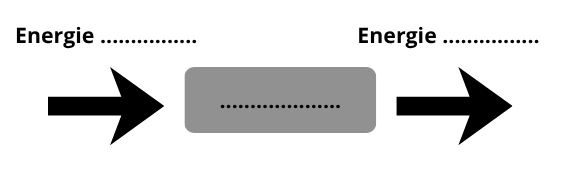
\includegraphics[width=5.3cm]{images/chaine d'énergie.png}\\
    \hline
    \rule{0pt}{2cm} Panneau solaire & & & & 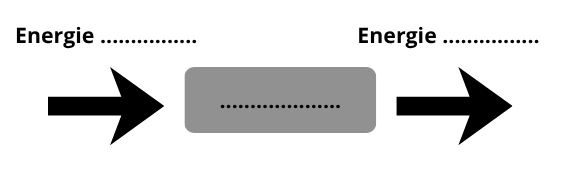
\includegraphics[width=5.3cm]{images/chaine d'énergie.png}\\
    \hline
    \rule{0pt}{2cm} Centrale hydraulique & & & & 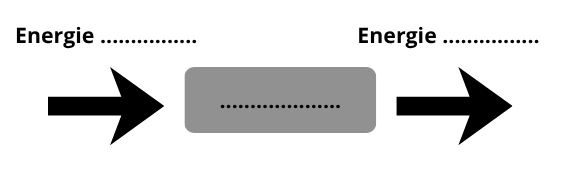
\includegraphics[width=5.3cm]{images/chaine d'énergie.png}\\
    \hline
    \rule{0pt}{2cm} Centrale nucléaire & & & & 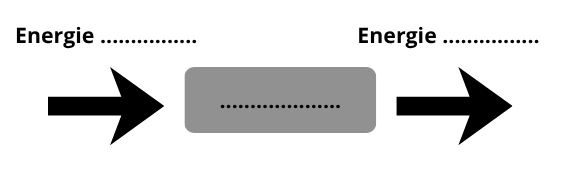
\includegraphics[width=5.3cm]{images/chaine d'énergie.png}\\
    \hline
    \rule{0pt}{2cm} Centrale thermique & & & & 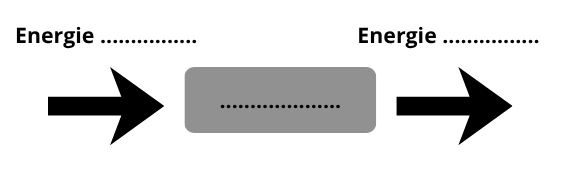
\includegraphics[width=5.3cm]{images/chaine d'énergie.png}\\
    \hline
\end{tabular}
\end{center}

\begin{enumerate}
    \item Explique la différence entre une énergie renouvelable et une énergie non renouvelable.

    \item Quelle est la source d'énergie la plus utilisée pour produire l'électricité en France en 2024 ? Et dans le monde ?

    \item Calcule le pourcentage d'énergies fossiles utilisées pour produire l'électricité dans le monde en 2024.

    \item Pourquoi est-ce un problème ?

    \item La France émet-elle beaucoup de CO\textsubscript{2} pour produire son électricité ? Justifie ta réponse.
\end{enumerate}

\end{document}

